

\begin{frame}
	\frametitle{Beyond Costs: The Triple Bottom Line}

    
	\centering
	\begin{itemize}
		\item Prosperity
		\item Direct costs and revenues
		\item Indirect costs and revenues
		\item Valuable functionality
		      
		\item People
		\item Job creation
		\item Equity
		\item Community/ lifestyle alignment
		      
		\item Planet
		\item Carbon emissions
		\item Ecosystem services
		\item Natural capital
	\end{itemize}
	
\includegraphics[width=0.9\linewidth]{figs/img0023.png}
	
\includegraphics[width=0.9\linewidth]{figs/img0024.png}
	
\includegraphics[width=0.9\linewidth]{figs/img0025.png}
	
\end{frame}


\begin{frame}
	\frametitle{Design for Value: Research Questions}
	\begin{itemize}
		\item Results-Oriented
        \begin{itemize}
    		\item What design optimizes WEC/system net value?
    		\item How does power matrix affect WEC/system value?
    		\item How do the above change for different grids?
        \end{itemize}
		      
		\item Methodological
        \begin{itemize}
    		\item What metrics are relevant?
    		\item What effects are important?
    		\item How to incorporate WEC design into grid model?
    		\item How to incorporate grid into WEC design optimization?
        \end{itemize}
	\end{itemize}
	
\end{frame}


\begin{frame}
	\frametitle{What metrics are relevant? Levelized Cost \& Value}
	Project levelized cost 
	(min revenue to offset costs)%PartTitle: =
	Project levelized viability 
	(if revenue offsets costs)%PartTitle: =
	System levelized cost
	(cost sum for all projects)
	
\end{frame}


\begin{frame}
	\frametitle{What effects are important?}
	\begin{itemize}
		\item Historical grid data:
		\item Due to hourly variation, wave had 7.5 \$/MWh higher value than solar (but wave costs >800 \$/MWh while solar costs 36 \$/MWh)
		\item Prior grid models incorporating WECs:
		\item WEC capacity factor and its standard deviation are important
		\item Due to seasonal variation, at 25\% CF, WECs are viable at 4x the cost of wind/solar; 50\% 5x; 75\% 7x
		\item Avoided capital costs >> avoided operating costs
	\end{itemize}
	
\end{frame}



\begin{frame}
	\frametitle{Optimization Structure}
	
	\centering
	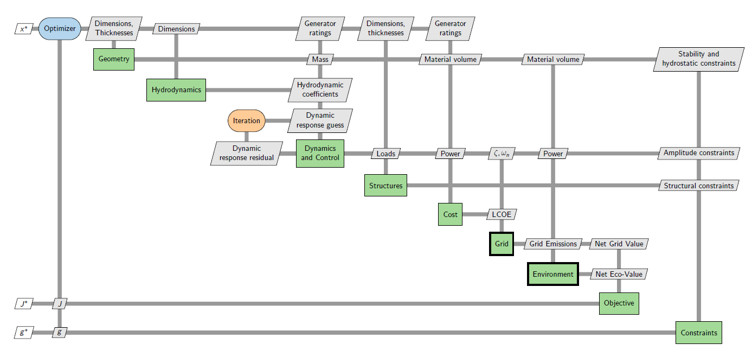
\includegraphics[width=0.9\linewidth]{figs/img0026.png}
	McCabe, Dietrich, Yang, Long, Kuan, Buccino, Liu, and Haji. “WEC optimization to maximize grid economic value and avoided emissions.” University Marine Energy Community Conference, August 2025, Corvallis OR.
	
\end{frame}


\begin{frame}
	\frametitle{Methods for Modeling the Grid}
	\begin{itemize}
		\item Accuracy
		      
		\item Compute time
		      
		\item Capacity Expansion Model (CEM)
		\item Find energy resource mix to minimize investment cost
		\item Linear program, can have millions of design variables
	\end{itemize}
	
\end{frame}


\begin{frame}
	\frametitle{3 ways to include grid in WEC design optimization}
	\begin{itemize}
		\item McCabe, Dietrich, Liu, and Haji 2023
	\end{itemize}
	
	CEM run ~100 times, design optimization is slow
	
	CEM run (fidelity)# intermediate metrics times, design optimization is fast, requires creating a WEC reduced order dynamic model
	
	CEM run once, design optimization is fast, but assumes WECs do not  affect the LP optimal basis
	
\end{frame}


\begin{frame}
	\frametitle{Challenges of grid model integration}
	
	\centering
	\begin{itemize}
		\item Representation of variability
		      \begin{itemize}
		      	\item Time series vs power matrix requires conversion
		      	\item Avoided operational costs have clear mapping
		      	\item Avoided capital costs don’t map to either
		      \end{itemize}
		\item WEC reduced order dynamic model
		      \begin{itemize}
		      	\item Power limit
		      	\item Power limit, natural frequency, damping ratio
		      	\item Power limit, pole/zero representation
		      	\item Power limit, hydrodynamics-based representation
		      	\item Polynomial / other black box
		      \end{itemize}
	\end{itemize}
	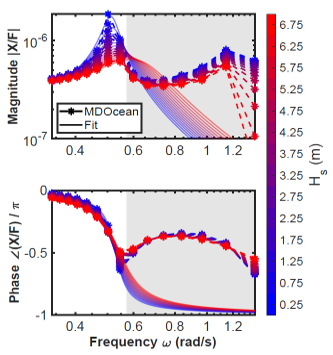
\includegraphics[width=0.9\linewidth]{figs/img0027.png}
	
\end{frame}

\begin{frame}
	\frametitle{Agenda}
	\AgendaSlide{Results}
\end{frame}


\begin{frame}
	\frametitle{Preliminary Results: Price Taker and Wave Binning}
	
	\centering
	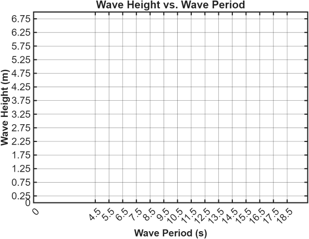
\includegraphics[width=0.9\linewidth]{figs/img0028.png}
	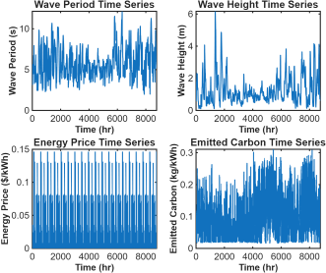
\includegraphics[width=0.9\linewidth]{figs/img0029.png}
	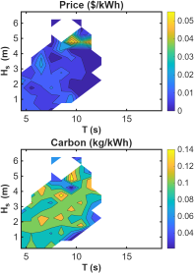
\includegraphics[width=0.9\linewidth]{figs/img0030.png}
	
\end{frame}


\begin{frame}
	\frametitle{Preliminary Results: CEM with Reduced Order Dynamics}
	
	\centering
	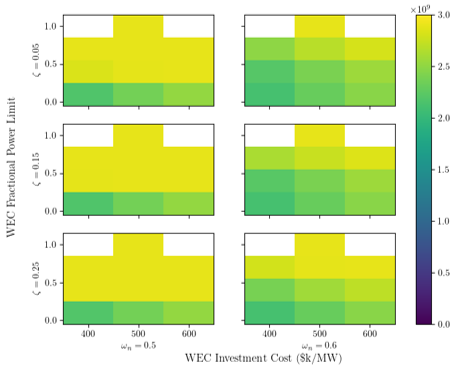
\includegraphics[width=0.9\linewidth]{figs/img0031.png}
	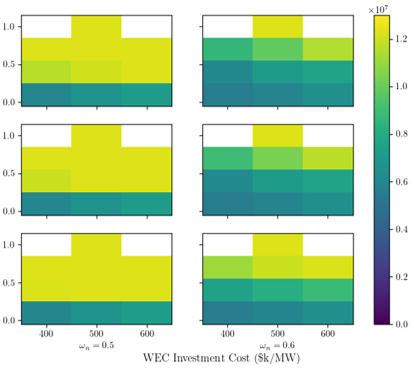
\includegraphics[width=0.9\linewidth]{figs/img0032.png}
	\begin{itemize}
		\item System Cost (\$)
		      
		\item CO2 Emissions (metric tonnes)
		      
		\item McCabe, Dietrich, Yang, Long, Kuan, Buccino, Liu, and Haji. “WEC optimization to maximize grid economic value and avoided emissions.” University Marine Energy Community Conference, August 2025, Corvallis OR.
	\end{itemize}
	
\end{frame}



\begin{frame}
	\frametitle{Systems Tensions}
	\begin{itemize}
		\item System boundary: insight, standardization
		      
		\item Disciplinary coupling: completeness, complexity
		      
		\item Model tradeoffs:           accuracy, intuition, dev+compute time
		      
		\item Uncertainty:           quantification, interpretation
	\end{itemize}
	
\end{frame}



